\section{Présentation du Projet}
L'état de dégradation des chaussées peut avoir un fort impact pour les usagers
et l'environnement. Ce projet a pour objectif de développer une solution
informatique pour améliorer les conditions de conduites face aux routes mal
entretenues.

\subsection{Enjeux}

-Sécurité (Dégradation rapide)
-Confort (Dégradation rapide)
-Cout
-Pollution
-Compétitivité

\subsection{Mise en oeuvre}
Etant donné l'étendue des réseaux routiers et leur rapide évolution, mobiliser
une équipe de personnel d'entretien afin de parcourir l'ensemble des routes, de
façon régulière, ayant pour mission de repérer et réparer les dégradations
n'est pas une
solution viable en terme de coût financier et environnemental. De plus, cette
méthode ne fournirait pas nécessairement de bons résultats puisque certaines
dégradations pourraient ne pas être vues ou tout simplement négligées par les
ouvriers.\\

\begin{figure}[H]
    \centering
    \begin{tikzpicture}[>=stealth,yscale=2,xscale=1.4]
        % Nodes
        \node(conducteur) at (0,0)[rectangle,draw,text centered,align=center]
        {Conducteur};
        \node(app) at (5,0)[rectangle,draw,text centered,align=center]
        {Application};
        \node(entretien) at (10,0)[rectangle,draw,text centered,align=center]
        {Ouvrier voiries};
        % Links
        \draw[-] (conducteur) -- (app);
        \draw[-] (app) -- (entretien)
    \end{tikzpicture}
    \caption{Description du fonctionnement du système}
    \label{analyse}
\end{figure}

Afin d'améliorer les conditions de conduites, toute dégradation de la chaussée
doit être signalée au plus vite au personnel chargé de l'entretien. Le
personnel peut être prévenu grâce à une notification provenant d'une
application pour smartphone.\\

La détection de défauts sur les infrastructures routières peut être réalisée
grâce à une analyse de données reccueillies sur les chaussées. Sachant que
l'état d'une chaussée peut se dégrader rapidement, ces données doivent être
recueillies régulièrement. On peut donc envisager que la collecte de données
soit réalisée de façon participative au travers de conducteurs volontaires en
utilisant une application pour smartphone.\\

\begin{figure}[H]
    \centering
    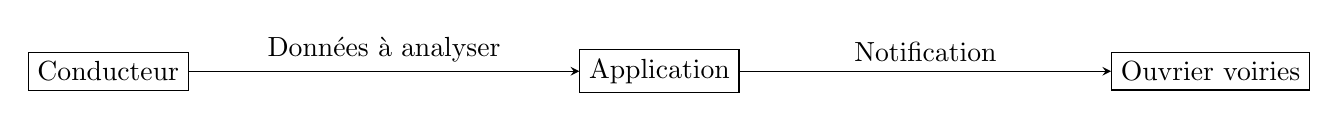
\begin{tikzpicture}[>=stealth,yscale=2,xscale=1.4]
        % Nodes
        \node(conducteur) at (0,0)[rectangle,draw,text centered,align=center]
        {Conducteur};
        \node(app) at (5,0)[rectangle,draw,text centered,align=center]
        {Application};
        \node(entretien) at (10,0)[rectangle,draw,text centered,align=center]
        {Ouvrier voiries};
        % Links
        \draw[->] (conducteur) -- (app) node[midway,above]{Données à analyser};
        \draw[->] (app) -- (entretien) node[midway,above]{Notification};
    \end{tikzpicture}
    \caption{Description du fonctionnement du système (Analyse)}
    \label{analyse}
\end{figure}

Le traitement

\begin{figure}[H]
    \centering
    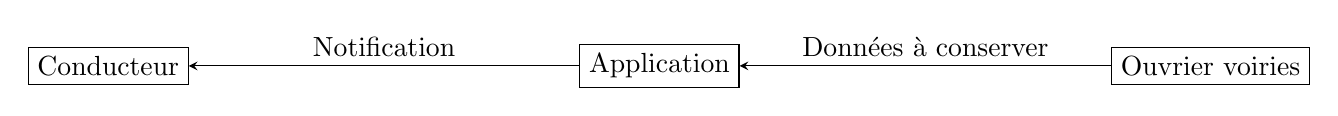
\begin{tikzpicture}[>=stealth,yscale=2,xscale=1.4]
        % Nodes
        \node(conducteur) at (0,0)[rectangle,draw,text centered,align=center]
        {Conducteur};
        \node(app) at (5,0)[rectangle,draw,text centered,align=center]
        {Application};
        \node(entretien) at (10,0)[rectangle,draw,text centered,align=center]
        {Ouvrier voiries};
        % Links
        \draw[<-] (conducteur) -- (app) node[midway,above]{Notification};
        \draw[<-] (app) -- (entretien) node[midway,above]{Données à conserver};
    \end{tikzpicture}
    \caption{Description du fonctionnement du système (Collecte)}
    \label{collecte}
\end{figure}